\documentclass[a4paper,12pt,language=finnish,version=final,hidechapters=true,includereferences=false,realtimesnewroman=false,sharelatex=true,emptyfirstpages=true,minted=true]{utuftthesis}
\setcounter{secnumdepth}{2}
\setcounter{tocdepth}{2}

%%
%% Minted
%%

\setminted{
breaklines,
baselinestretch=1.1,
frame=lines,
linenos
}
\usemintedstyle{monokai}
\usepackage{xcolor}

\addbibresource{Bibliografia.bib}
\begin{document}

\pubyear{2022}

\pubmonth{6}

\publab{Tietotekniikka}

\publaben{Laboratory Name}

\pubtype{tkk}
\title{Tilanhallinta React.js-pohjaisessa web-sovelluksessa}
\author{Vili Ståhlberg}

\maketitle
\keywords{React, React Hooks, web-sovellukset, tilanhallinta, Flux-arkkitehtuuri, Redux}
\begin{abstract}
Yhden sivun web-sovellukset ovat uudistaneet verkkokehittämistä uusilla innovatiivisilla ratkaisuilla. Perinteisiin monen sivun verkkosivustoihin verrattuna JavaScript-pohjaiset yhden sivun web-sovellukset mahdollistavat kustannustehokkaamman ja vuorovaikutteisemman kokemuksen käyttäjälle. Jotta tämä olisi mahdollista, tulee sovelluksessa olla yksi tai useampi tila, joka voi muuttua esimerkiksi vastauksena käyttäjän antamaan syötteeseen. Tässä tutkielmassa tarkastellaan web-sovelluksen tilaa sekä sen hallintaa Metan kehittämän React JavaScript -kirjaston näkökulmasta. Tutkielmassa käsitellään tilanhallintaan liittyviä perusoperaatioita, haasteita sekä hyödyllisiksi ja toimiviksi todettuja menetelmiä ja työkaluja. 

Tutkielma on toteutettu kirjallisuuskatsauksena. Tutkielmassa käsitellään tilanhallinnassa tyypillisesti esiintyviä ongelmia sekä tilanhallinnan menetelmiä. Esitettyihin ongelmiin pyritään tutkielman aikana esimerkkien johdattelemana esittämään ratkaisuja tilanhallinnan menetelmien avulla.

Tutkielman johtopäätöksenä voidaan todeta, että modernien web-sovellusten tilanhallintaan liittyviin ongelmiin on olemassa tilannekohtaisia ratkaisuja, joita tutkielmassa eritellään. Menetelmiä ja ratkaisuja ovat esimerkiksi tilanhallintaan suunnatut ulkoiset kirjastot sekä komponenttien kokoonpanon laatiminen tietyllä tavalla. Yhtä oikeaa ratkaisua ei ole. Sopivan menetelmän valinta ja käyttöönotto perustuu pitkälti sovelluksen monimutkaisuuteen ja laajuuteen. Menetelmän toimivuuden lisäksi sovelluksen kehittäjän pohdittavaksi jää sovelluksen kokoluokalle ja monimutkaisuudelle sopivan ratkaisun valinta.
\end{abstract}

% Ehkä viimeisessä kappaleessa voisi vielä jotenkin
% todeta -- vähän rautalangasta vääntämällä -- että
% tutkielman tuloksena myös eritellään sitä, mikä
% tilanhallinta ratkaisu sopii mihinkin tilanteeseen.
% Muuten on ehkä vaarana se, että annetaan tiivistelmän 
% lukijalle vähän lattea "ratkaisuja on monia erilaisia"
% -mielikuva ilman aiheen syvempää käsittelyä, mikä ei tietysti
% tee tutkielman viimeisille luvuille oikeutta
%
% -SR


% empty pagestyle for table of contents etc.
% otherwise you'll get simple page style with roman page numbers
\pagestyle{empty}

% mandatory
\tableofcontents

% if you want a list of figures
%\listoffigures

% if you want a list of tables
%\listoftables

% 'list of acronyms'
%   - you may not need this at all
%   - create a chapter called List Of Acronyms (or whatever), which
%     should contain all your acronym definitions, e.g. 
%     \chapter{List Of Acronyms} 
%   - the secnumdepth trickery is needed because acronyms are as a
%     standard chapter and we are faking '\listofacronyms'
%
%\setcounter{secnumdepth}{-1}
%\input{your acronym chapter's file name}
%\setcounter{secnumdepth}{2}% setup page numbering, page counter, etc.%

\chapter{Johdanto} \label{johdanto}

%Tutkimuskysymys 1: Minkälaisia ongelmia tilanhallintaan liittyy?
%Tutkimuskysymys 2: Minkälaisia käytännölliseksi todettuja keinoja ja työkaluja tilanhallinnan helpottamiseksi on olemassa?

Yhden sivun web-sovellukset (engl. single-page application) ovat tuoneet mukanaan uudenlaisen tavan luoda käyttäjäystävällisiä ja käytännöllisiä verkkoympäristöjä ja sovelluksia. Perinteisissä monen sivun verkkosivustoissa ilmenneitä sekä suorituskykyyn että käyttökokemukseen vaikuttaneita ongelmia ja puutteita on onnistuttu ratkaisemaan yhden sivun web-sovelluksien avulla. Tyypillinen perinteisiin monen sivun verkkosivustoihin liittynyt ongelma on esimerkiksi tarpeettoman monet palvelinpyynnöt, jolloin jokaisella sivun latauskerralla käyttäjän selain lataa joko osittain tai kokonaan täysin samat resurssit palvelimelta. Yhden sivun web-sovelluksessa sivu käytännössä ladataan kerran, ja täytetään tarvittaessa uudelleen dynaamisesti. Tällöin käyttäjän ei tarvitse jokaisella latauskerralla noutaa resursseja uudestaan.

Tilanhallinta on yksi keskeisimpiä web-sovelluksen kehittämisessä vastaan tulevia kysymyksiä. Tilan on oltava saatavilla sitä tarvitsevissa komponenteissa, ja sitä on tietyissä tapauksissa päästävä muuttamaan sovelluksen eri osista käsin. Sulavan kehitysprosessin edistämiseksi kehittäjän tulee huomioida nämä asiat jo komponenttien suunnitteluvaiheessa. Sovelluksen kasvaessa suuremmaksi komponentit tyypillisesti etääntyvät toisistaan huomattavasti, jolloin alkuperäinen ratkaisu ei enää välttämättä ole käytännöllinen tai edes toimiva. Kokenut web-sovelluksiin perehtynyt kehittäjä tunnistaa ja osaa ennakoida tilanhallintaan liittyviä ongelmia sekä ratkaista niitä myös jälkikäteen.

Tässä tutkielmassa on määrä esittää lukijalle holistinen näkemys tilanhallinnasta. Tilanhallintaa tarkastellaan Metan kehittämän React JavaScript -kirjaston näkökulmasta. Tutkimuskysymykset ovat: (1) \textit{Minkälaisia ongelmia tilanhallintaan liittyy?} ja (2) \textit{Minkälaisia käytännölliseksi todettuja keinoja ja työkaluja tilanhallinnan helpottamiseksi on olemassa?}

Tutkielma on toteutettu kirjallisuuskatsauksena. Tutkittavaan aiheeseen liittyvää aineistoa on haettu informaatioteknologian kannalta olennaisista tietokannoista, kuten Web of Science, ACM sekä IEEE/IEE. Tutkielman luvussa \ref{reactjs} käsitellään React-kehityksen kannalta olennaisia käsitteitä. Luvussa \ref{tilanhallinta} avataan tilanhallinnan avainkäsitteet ja esitetään konkreettisia esimerkkejä tilanhallinnan perusoperaatioista. Tilanhallinnassa usein esiintyviä ongelmia käsitellään luvussa \ref{Tilanhallinnan ongelmat} esimerkkien kautta. Luvussa \ref{Tilanhallinnan menetelmät} käsitellään tilanhallinnan menetelmiä ja niiden käyttötapauksia. Lisäksi menetelmiä sovelletaan luvussa \ref{Tilanhallinnan ongelmat} käsiteltyihin ongelmiin. Tutkielman johtopäätökset esitetään lopuksi luvussa \ref{Johtopäätökset}.
\chapter{React.js} \label{reactjs}
Dynaamisen komentokieli JavaScriptin suosion kasvun myötä syntyivät yhden sivun web-sovelluksien kehittämistä varten suunnitellut JavaScript-kehykset (engl. framework) ja -kirjastot (engl. library). Tällaisia maailmanlaajuisesti käytettyjä ja käytännöllisiksi tunnustettuja kehyksiä ja kirjastoja ovat esimerkiksi Angular JS, Vue.js ja React.js. Näistä kolmesta jälkimmäisin on tutkielman kirjoitushetkellä kasvanut maailmanlaajuisesti suosituimmaksi työkaluksi web-sovelluksien kehityksessä \cite{stackoverflowsurvey}.

React.js on Metan kehittämä ilmainen avoimen lähdekoodin JavaScript-kirjasto. Meta tunnettiin aiemmin nimellä Facebook. React kehitettiin yhden sivun web-sovelluksien kehittämistä varten. Kirjastoa ylläpitää aktiivisesti Metan lisäksi useasta henkilöstä ja yrityksestä koostuva yhteisö \cite{reactdocsteam}. Kirjastona React ottaa muita vastineitaan vähemmän kantaa erilaisten toiminnallisuuksien toteutustapoihin. Tästä syystä Reactin ympärille on muodostunut laaja kehittäjäyhteisö, joka kehittää ja julkaisee erilaisia kirjastoja, toteutustapoja ja ratkaisuja tyypillisiin ongelmiin \cite{rawatmahajan}. Tästä laajasta valikoimasta yksittäinen kehittäjä voi valita itselleen tai projektille soveltuvimman toteutustavan. Esimerkiksi reitittäminen toiminnallisuutena, joka on hyvin tyypillinen yhden sivun web-sovelluksessa, ei sisälly React-pakettiin, vaan löytyy muiden Reactin kehittäjätiimin ulkopuolisten kehittäjien julkaisemina ja ylläpitäminä kirjastoina. Vastaesimerkkinä laajemmin kantaa ottavasta JavaScript-kehyksestä on Angular JS, jossa esimerkiksi reitittäminen sisältyy kehykseen valmiina ominaisuutena. Vaikka React jättää monimutkaisemmat toiminnot kehittäjän harkintakyvyn varaan, on Reactissa kuitenkin selkeät raamit kehittämiselle. Esimerkiksi funktionaalisuudesta ja sovelluksen komponenttipohjaisuudesta ei voi Reactin käytössä välttyä.

%%
%% JSX
%%

\section{JSX}
\label{JSX}

JavaScript XML (JSX) on hyvin yleisesti React-sovelluksissa käytetty JavaScript-syntaksin jatke. JSX mahdollistaa React-elementtien luomisen deklaratiivisella ja yksinkertaistetulla syntaksilla. Visuaalisesti JSX muistuttaa pitkälti HTML-syntaksia.
\inputminted[bgcolor=black]{jsx.py:JsxLexer -x}{listaukset/jsx.js}
Myös lausekkeiden upottaminen on JSX:n avulla mahdollista. Sisällyttämällä minkä tahansa JavaScript-standardien mukainen lausekkeen aaltosulkeiden sisälle voidaan hyödyntää esimerkiksi muuttujaa tiedon esittämisessä. \cite{reactdocsjsx}
\inputminted[bgcolor=black]{jsx.py:JsxLexer -x}{listaukset/jsxexpression.js}

JSX:n käyttö ei ole kuitenkaan edellytys Reactin käytölle. React-sovelluksen kehittäminen onnistuu myös kirjoittamalla standardien mukaista Javascript-koodia. Tällöin React-elementin määritteleminen tulee tehdä Reactiin sisällytetyllä \texttt{createElement}-metodilla. \cite{reactdocswithoutjsx}
\inputminted[bgcolor=black]{jsx.py:JsxLexer -x}{listaukset/withoutjsx.js}
Vaikka JSX:n käyttö ei ole pakollista, on se hyvin suotavaa React-sovelluksen kehittämisessä.

%%
%% Komponentit
%%

\section{Komponentit}
\label{Komponentit}

Komponentit ovat oleellinen osa React-sovellusta. Ne toimivat rakennuspalikoina, joita yhdistelemällä sovellus muodostetaan \cite{reactdocscomponents}. Komponenttien avulla sovelluksen käyttöliittymä on mahdollista pilkkoa mielivaltaisen pieniin osiin, joita voidaan oikein toteutettuna käyttää toistuvasti sovelluksen eri osissa \cite{reactdocscomponents}. Komponentin pilkkominen osiin tuo erityisesti laajoihin kokonaisuuksiin selkeyttä ja läpinäkyvyyttä. Komponentin uusiokäytettävyyttä taas pidetään yleisesti hyvänä ominaisuutena. Uusiokäytettävien komponenttien suunnittelu ja kehitys vie aluksi aikaa, mutta säästää lopulta laajoissa sovellushankkeissa runsaasti aikaa ja resursseja \cite{holzmann}. Jos sovelluksessa on paljon toiminnaltaan samankaltaisia elementtejä tai saman ominaisuuden käyttötapauksia, voidaan kertaalleen laadittua komponenttia käyttää uudelleen useassa eri paikassa. Tällöin vältytään kyseisen komponentin kirjoittamiselta uudelleen joko osittain tai täysin.

Komponentin määrittelyyn on kaksi eri lähestymistapaa. Yksinkertaisin tapa määritellä komponentti on kirjoittaa (1) JavaScript-funktio. \cite{reactdocscomponents}
\inputminted[bgcolor=black]{jsx.py:JsxLexer -x}{listaukset/functioncomponent.js}
Komponentin voi toisaalta määritellä myös perusteellisemmin ES6-standardin mukaisella (2) JavaScript-luokalla. \cite{reactdocscomponents}
\inputminted[bgcolor=black]{jsx.py:JsxLexer -x}{listaukset/classcomponent.js}
Kun komponentti on määritelty, se voidaan ottaa käyttöön yksinkertaisella HTML-syntaksia muistuttavalla React-elementillä \texttt{<Komponentti />}. Elementit renderöidään loogisesti niiden esitysjärjestyksessä. 
\inputminted[bgcolor=black,highlightlines={4-5},highlightcolor=darkgray]{jsx.py:JsxLexer -x}{listaukset/componentusage.js}
Molemmat määrittelytavat ovat Reactin näkökulmasta yhtä päteviä. Funktiokomponenttien suosio on kuitenkin lisääntynyt kehittäjien keskuudessa niiden julkaisusta lähtien \cite{twilio}. Jopa itse Reactin takana olevan kehitystiimin tavoitteena on asteittain siirtyä luokkakomponenteista funktiokomponentteihin ajan kuluessa. \cite{reactdocshooks}

%%
%% Props
%%

\subsection{Props}
\label{Props}

Props eli properties on keino antaa komponentille tietoa käytettäväksi JavaScript-olion muodossa \cite{reactdocscomponents}. Propsit muistuttavat hyvin pitkälti funktiolle annettavia parametreja. Eräs tyypillinen propsien käyttötapaus on tilan jakaminen komponentilta toiselle. Tätä käsitellään tarkemmin tutkielman luvussa \ref{Tilan jakaminen muille komponenteille}. 

%%
%% Elinkaari
%%

\subsection{Elinkaari}
\label{Elinkaari}

Jokaisella React-komponentilla on oma elinkaarensa (engl. lifecycle). Elinkaari alkaa komponentin renderöinnistä ja päättyy lopulta komponentin irrotukseen dokumenttioliomallista (engl. document object model) \cite{reactdocsstate}. Komponentin elinkaaren avulla on mahdollista ajoittaa tiettyjen toimintojen suorittamista eri ajankohtiin ja tapahtumiin sovelluksen käynnistyksestä alkaen \cite{reactdocsstate}. Kuvasta \ref{fig:lifecycle} nähdään, miten komponentin elinkaari etenee komponentin kiinnittymisestä irtoamiseen. Tuntemalla ja tiedostamalla komponentin elinkaaren kehittäjä voi tehdä sovellukseen merkittäviä optimointeja, joilla on suora vaikutus sovelluksen suorituskykyyn ja käytettävyyteen. 
\begin{figure}[h]
\centering 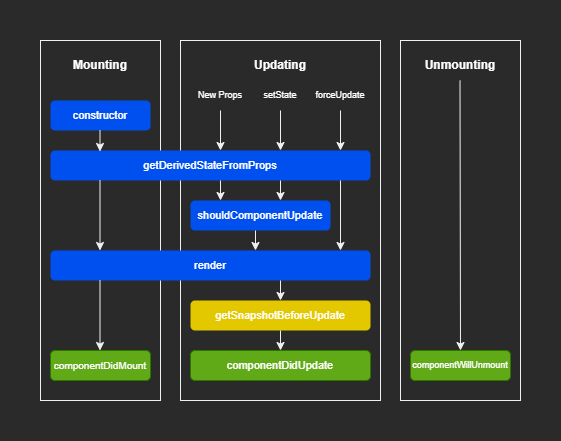
\includegraphics[width=1\textwidth]{kuvat/Elinkaari.png}
\caption{Graafinen esitys komponentin elinkaaresta.}
\label{fig:lifecycle} 
\end{figure}

%%
%% Tila
%%

\subsection{Tila}
\label{Tila}

Tila on läheisesti komponenttiin liittyvä käsite ja on tämän tutkielman näkökulmasta hyvin keskeisessä asemassa. Komponentilla voi olla yksi tai useampi tila, jota on mahdollista muuttaa esimerkiksi käyttäjän syötteen perusteella. Tilaa voidaan käyttää eri tarkoituksiin, kuten komponentin dynaamiseen esitystyyliin tai ehdolliseen näkyvyyteen. Mikäli komponentin palauttava \texttt{return}-lauseke on riippuvainen tilasta, joka voi muuttua, aiheutuu kuvan \ref{fig:component} mukaisesti kyseisen tilan muutoksesta komponentin päivittävä renderöinti \cite{reactandnative}. Käytännössä React vertaa edellistä DOM:in versiota nykyiseen ja suorittaa niiden osien päivittämisen, joihin muuttunut tilan arvo vaikuttaa. Tällöin vältytään koko sovelluksen päivittävältä renderöinniltä tilanteissa, joissa se ei ole ehdottoman tarpeellista. \cite{reactdocsrender}

\begin{figure}[h]
\centering 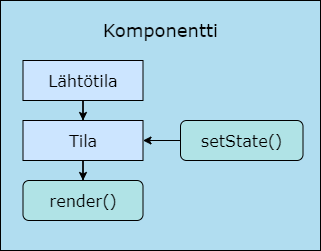
\includegraphics[width=0.5\textwidth]{kuvat/Komponentti.png}
\caption{Muutos tilassa aiheuttaa sitä käyttävän komponentin päivittävän renderöinnin.}
\label{fig:component} 
\end{figure}

%%
%% Hookit
%%

\section{Hookit}
\label{Hookit}

React julkaisi vuonna 2018 version 16.8 yhteydessä React Hooks -rajapinnan. Hookit ovat kokoelma erilaisia funktioita, jotka alkavat aina sanalla \texttt{use}. Hookit mahdollistavat React-komponentin ominaisuuksien käytön kirjoittamatta komponenttia luokkana \cite{reactdocshooks}. Esimerkkejä tällaisista ominaisuuksista ovat komponentin tilan määrittäminen ja päivittäminen sekä luvussa \ref{Elinkaari} mainitut elinkaarimetodit. Verrattuna luokkakomponentteihin funktiokomponentit yhdessä hookien kanssa ovat tyypillisesti helpommin luettavissa \cite[10]{buglreacthooks}. Ne myös vähentävät merkittävästi rutiininomaisen ja toistuvan koodin (engl. boilerplate code) kirjoittamista \cite{reactdocshooks} \cite[62]{reactandnative} \cite[11]{buglreacthooks}. Tutkielman myöhemmissä osissa tullaan käyttämään esimerkkeinä funktiokomponentteja yhdessä React Hooks -funktioiden kanssa luokkakomponenttien sijasta. 
\chapter{Tilanhallinta} \label{tilanhallinta}

Tila käsitteenä on yksi React-sovelluksen tärkeimpiä ominaisuuksia. Sovelluksen vuorovaikutteisuus ja intuitiivisuus parantavat käyttäjäkokemusta \cite{userexperience}. Jotta sovellus toimisi vuorovaikutteisesti käyttäjän kanssa, tulee sovelluksen reagoida ja muuttua erilaisten syötteiden mukaisesti. Syöte voi olla peräisin käyttäjältä, mutta se voi myös tulla esimerkiksi toisella palvelimella sijaitsevasta rajapinnasta. Luvussa \ref{Tila} esitetyn komponentin tilan käyttäminen on erinomainen tapa hallinnoida sovelluksen vuorovaikutteisuutta.

Tilanhallinnalla (engl. state management) viitataan toisaalta yksinkertaisesti tilan muuttamiseen, mutta myös tilan hallittavuuteen. Sovelluksen kasvaessa ja monimutkaistuessa kehittäjän tekemät tilanhallinnan ratkaisut korostuvat, jolloin keskinkertaiset ratkaisut vaativat jatkokehitystä tai ääritapauksessa jopa kokonaan korvaamista uudenlaisilla ratkaisuilla. Tässä luvussa perehdytään tarkemmin tilanhallinnan peruskäsitteisiin yksinkertaisten esimerkkien johdatuksella.

%%
%% Paikallinen tila
%%

\section{Paikallinen tila}
\label{Paikallinen tila}

Yksittäisen komponentin sisällä hallittua tilaa kutsutaan paikalliseksi tilaksi (engl. local state). Komponenttia, jolle on asetettu yksi tai useampi tila, kutsutaan tilalliseksi komponentiksi (engl. stateful component). Tila asetetaan komponentissa, jolloin oletuksena vain kyseisellä komponentilla on kyky käyttää tilaa. Tilan asettaminen funktiokomponentille tehdään Reactiin sisällytetyn \texttt{useState}-hookin avulla.

Uuden tilan asettaminen aloitetaan määrittelemällä uusi vakio ja kutsumalla \texttt{useState}-funktiota. \texttt{useState} palauttaa kaksi alkiota sisältävän taulukon (engl. array). Ensimmäinen alkio sisältää tilamuuttujan johon tila tallennetaan. Toinen alkio on funktio, jolla tilaa voidaan päivittää. \cite[64]{reactandnative}
\inputminted[bgcolor=black,highlightlines={2},highlightcolor=darkgray]{jsx.py:JsxLexer -x}{listaukset/counter.js}
Esimerkissä yksinkertaiseen laskurikomponenttiin muodostetaan destrukturointilauseke, jolla nimetään tilamuuttuja \texttt{count}, tilan päivittävä funktio \texttt{setCount} sekä asetetaan tilan lähtöarvo. Tilamuuttuja \texttt{count} sisältää tilalle asetetun arvon. Lähtöarvo annetaan \texttt{useState}-funktiolle parametrina, joka on tässä esimerkissä asetettu nollaksi.


%%
%% Tilan päivittäminen
%%

\section{Tilan päivittäminen}
\label{Tilan päivittäminen}

Tilan päivittäminen suoritetaan esimerkissä annetulla \texttt{setCount}-funktiolla. Funktion parametriksi annetaan haluttu päivitetty arvo.
\inputminted[bgcolor=black,highlightlines={5,7},highlightcolor=darkgray]{jsx.py:JsxLexer -x}{listaukset/counter2.js}
Esimerkissä jompaakumpaa nappia painamalla laukaistaan JavaScript ES6 -standardin mukainen nuolifunktio, joka asettaa tilalle uuden arvon vähentämällä tai lisäämällä edeltävään arvoon luvun yksi. Tilaa ei saa koskaan päivittää suoraan asettamalla sille uuden arvon. Päivittäminen tulee aina tehdä \texttt{useState}-hookille annetulla funktiolla. \cite{reactdocsstate}

%%
%% Tilan jakaminen muille komponenteille
%%

\section{Tilan jakaminen muille komponenteille}
\label{Tilan jakaminen muille komponenteille}

Jotta komponenttien jakaminen pienempiin itsenäisiin osiin olisi mahdollista, täytyy tiedon pystyä liikkumaan eri komponenttien välillä. Tilan jakaminen komponentilta toiselle tehdään luvussa \ref{Props} mainittujen propsien avulla:
\inputminted[bgcolor=black,highlightlines={6},highlightcolor=darkgray]{jsx.py:JsxLexer -x}{listaukset/counter3.js}
Esimerkissä laskurin toiminnallisuudesta vastaava komponentti \texttt{Counter} toteuttaa kaikki laskuriin liittyvän tilanhallinnan toimenpiteet. Se ei kuitenkaan ota kantaa suoraan miten laskurin lukuarvo tulisi esittää. Sen sijaan lukuarvo syötetään eteenpäin \texttt{Display}-komponentin käsiteltäväksi ja esitettäväksi rivillä 6:
\inputminted[bgcolor=black]{jsx.py:JsxLexer -x}{listaukset/display.js}

Reactin virallisesta dokumentaatiosta sekä aiemmin esitetyistä esimerkeistä ilmenee, että tieto liikkuu ylhäältä alaspäin komponenttien välillä. Tietovirta on siis yksisuuntaista \cite{reactdocsstate}. Tämän lisäksi propseina tietoa saanut komponentti ei välitä tiedon alkuperästä. Myöskään sillä ei ole merkitystä onko tieto jonkin toisen komponentin hallitsema tila vai yksinkertaisesti jokin käsin kirjoitettu mielivaltainen arvo. Komponentin näkökulmasta ainoastaan sillä on merkitystä, että tieto on saatavilla propsien muodossa.
\chapter{Tilanhallinnan ongelmat} \label{Tilanhallinnan ongelmat}

Sovelluksen kasvaessa suuremmaksi ja monimutkaisemmaksi alkaa tilanhallinnassa esiintymään lähestulkoon väistämättä erilaisia esteitä ja vaikeuksia \cite{kentcdodds1} \cite{ivakop}. Tilanhallinnan ongelmat vaikuttavat hyvin konkreettisesti sovelluksen skaalautuvuuteen ja muutosten tekemiseen tulevaisuudessa. Mikäli tilanhallintaa ei huomioida alusta alkaen, siitä johtuvat ongelmat korostuvat \cite{discussion}.

Tässä luvussa käsitellään kahta tyypillistä tilanhallinnan ongelmaa esimerkkien johdattelemana. Tutkielmaan on tarkoituksella valittu käsiteltäväksi nämä kaksi ongelmatyyppiä, sillä muut tilanhallinnassa esiintyvät ongelmat useimmiten juurtavat juurensa näistä kahdesta ongelmatyypistä.

%%
%% Tilan sijainti komponenttipuussa
%%

\section{Tilan sijainti komponenttipuussa}
\label{Tilan sijainti komponenttipuussa}

Tila on aina sidottu sitä hallinnoivaan komponenttiin. Tästä johtuen kyseisen tilallisen komponentin sijainti komponenttipuussa on erityisen tärkeä, mikäli kyseistä tilaa tarvitaan myös sovelluksen muissa komponenteissa.

%%
%% Kaukana oleva käyttökohde
%%

\subsection{Kaukana oleva käyttökohde}
\label{Kaukana oleva käyttökohde}
Luvussa \ref{Tilan jakaminen muille komponenteille} käsitelty tilan jakaminen lapsikomponentille voi alkaa käymään hyvin työlääksi ja sekavaksi, jos tilaa hyödyntävä lapsikomponentti sijaitsee komponenttipuussa huomattavan monen komponenttikerroksen verran alempana. Prop drilling on epävirallinen nimitys prosessista, jossa kehittäjä jakaa komponentin tilaa usean komponenttikerroksen läpi saavuttaakseen lopulta tilaa hyödyntävän komponentin. Tällaisessa tilanteessa kyseessä olevan kahden komponentin väliin jäävät komponentit eivät itse tarvitse kyseistä tilaa. Tällöin ne ainoastaan kuvan \ref{fig:drilling} mukaisesti vastaanottavat sen propseina jakaakseen sen eteenpäin seuraavalle komponentille. \cite{kentcdodds2}
\begin{figure}[h]
\centering 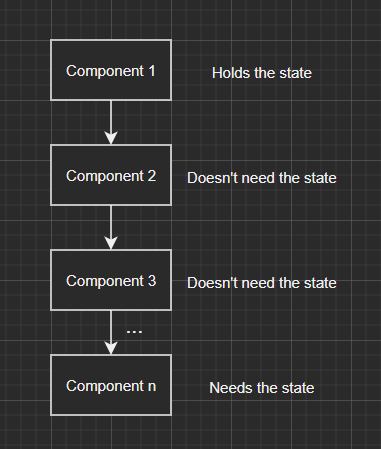
\includegraphics[width=0.5\textwidth]{kuvat/Prop Drilling.png}
\caption{Tilaa voidaan joutua jakamaan usean komponenttikerroksen läpi vaikka väliin jäävät komponentit eivät sitä tarvitse.}
\label{fig:drilling} 
\end{figure}

Sen lisäksi, että prop drilling voi tehdä tilan jakamisesta työlästä, voi myös esimerkiksi mahdollisten muutoksien tekeminen tulevaisuudessa hankaloitua. Mikäli tilaa hallitseva komponentti siirretään tai poistuu kokonaan käytöstä, voi kehittäjä joutua ääritapauksessa purkamaan koko tilaa jakavien komponenttien putken.

%%
%% Jakaminen samalla tasolla
%%

\subsection{Jakaminen samalla tasolla}
\label{Jakaminen samalla tasolla}

Luvussa \ref{Tilan jakaminen muille komponenteille} todettiin, että tieto liikkuu React-sovelluksen komponenttien välillä yksisuuntaisesti ylhäältä alaspäin. Kuitenkin esimerkiksi komponentteja pilkkoessa pienempiin osiin voi kehittäjällä tulla vastaan tilanne, jossa samassa tasossa sijaitsevat komponentit tarvitsevat viereisessä komponentissa hallinnoitua tilaa.
\inputminted[bgcolor=black]{jsx.py:JsxLexer -x}{listaukset/horizontalstate.js}
Esimerkissä esitetty laskuri sisältää kaksi komponenttia, joista \texttt{Counter} sisältää laskurin toiminnallisuuden. \texttt{Display} vastaa laskurin tilan arvon näyttämisestä käyttäjälle. Komponentit ovat komponenttipuussa samalla tasolla, joten tilaa ei voi suoraan jakaa \texttt{Counter}-komponentista \texttt{Display}-komponentin näytettäväksi.

%%
%% Monimutkainen tila
%%

\section{Monimutkainen tila}
\label{Monimutkainen tila}

Yksinkertaisen laskurin ylläpitämän tilan \texttt{count} lukuarvon ylläpitäminen ei ole hankalaa. Laskurin tilan arvoa on helppo muuttaa lisäämällä tai vähentämällä edellisestä arvosta luvun yksi. Laskuria on myös suhteellisen helppoa jatkokehittää esimerkiksi lisäämään tai vähentämään arvoja käyttäjän syötteen perusteella. Jos kyseessä on kuitenkin laskuria huomattavasti monimutkaisempi tietotyyppi tai -rakenne, voi tilan päivittäminen hankaloitua ja täten muuttua jatkokehityksen näkökulmasta huomattavasti työläämmäksi.
\inputminted[bgcolor=black,samepage]{jsx.py:JsxLexer -x}{listaukset/complexstate.js}
Esimerkissä tila \texttt{state} on JavaScript-olio, joka sisältää merkkijonon, kokonaisluvun sekä mielivaltaisen määrän olioita sisältävän taulukon. Esimerkissä käytettyä ES6-standardin mukana tullutta \texttt{spread}-operaattoria käyttämällä päivittäminen on vielä suhteellisen helppoa. Jos kuitenkin halutaan päivittää tilassa esiintyvää arvoa monimutkaisemmalla logiikalla tai useasti toistuvalla tavalla, alkaa tilan päivittämisestä tulla kasvavassa määrin työläämpää. Kehittäjä voi tällaisessa tilanteessa joutua toistuvasti kirjoittamaan logiikaltaan hyvin samankaltaista koodia, jossa ei ole hyödynnetty abstraktiota juuri ollenkaan. Tällainen kehittäminen ei noudata ohjelmistokehityksessä hyväksi todettua DRY-periaatetta (sanoista don't repeat yourself) \cite{dry1} \cite{dry2}.
\input{menetelmät}
\chapter{Johtopäätökset} \label{Johtopäätökset}

% voisi aloittaa luvun vielä kertaamalla tilanhallinnan käsitteen
% ja sen merkityksen
% -SR

Tässä tutkielmassa käsiteltiin tilaa sekä tilanhallintaa. Tila tarkoittaa sovellukseen tallennettua tietoa, joka voi muuttua esimerkiksi reagoimalla käyttäjän syötteeseen. Tilanhallinnalla siis tarkoitetaan tilan käyttöön, esittämiseen sekä päivittämiseen tarvittavia toimenpiteitä ja ratkaisuja. Tutkielmassa käsiteltiin tilanhallintaan liittyviä ongelmia sekä tilanhallinnan menetelmiä, joita sovellettiin tyypillisiin tilanhallinnan ongelmiin esimerkkien avulla.

%Tutkimuskysymys 1: Minkälaisia ongelmia tilanhallintaan liittyy?
Tutkielmassa käsiteltyjen asioiden nojalla voidaan todeta tilanhallinnan olevan hyvin keskeinen käsite React-sovelluksen kehityksessä. Tilanhallintaan liittyviä ongelmia on erityyppisiä ja ne ilmenevät sovelluksissa eri tavoin, riippuen esimerkiksi sovelluksen toiminnallisuusvaatimuksien monimutkaisuudesta sekä laajuudesta. Ongelmat juontavat juurensa tyypillisesti joko tilan jakamisesta komponenttien välillä tai monimutkaistuneista tietotyypeistä. Mikäli tilanhallintaa ei huomioida jo sovelluksen suunnitteluvaiheessa, sovelluksessa ilmenee tutkielmassa käsiteltyjä ongelmia hyvin suurella todennäköisyydellä. 

%Tutkimuskysymys 2: Minkälaisia käytännölliseksi todettuja keinoja ja työkaluja tilanhallinnan helpottamiseksi on olemassa?
Tutkielman pohjalta voidaan myös todeta, että on olemassa useita varteenotettavia tilanhallinnan menetelmiä, joista jokaisella on omat käyttötapauksensa. Tilanhallintaan ei ole siis olemassa yhtä ainutta oikeaa ratkaisua. Luvussa \ref{Tilan nostaminen} käsitelty tilan nostaminen komponenttipuussa tasoa korkeammalle on yksinkertainen ja nopea ratkaisu tilan jakamiseen kahdelle samalla tasolla sijaitsevalle komponentille. Luvussa \ref{useContext} käsitellyn kontekstin käyttöönotto voi olla käytännöllinen ratkaisu tilanhallintaan, jos tilaa tarvitaan huomattavan monessa eri komponentissa. Toisaalta konteksti voi olla pienemmissä sovelluksissa turhan järeä ratkaisu, jolloin luvussa \ref{Kokoonpano ja periminen} käsitelty kokoonpano voi olla yksinkertaisempi vaihtoehto. Mikäli sovelluksen arvioidaan olevan toiminnallisuudeltaan monimutkainen ja kehityksessä on mukana useita kehittäjiä, on esimerkiksi tutkielman luvussa \ref{useReducer} käsiteltyjen reducerien käyttöönotto tällaisessa tapauksessa suotavaa. Myös luvussa \ref{Redux-kirjasto} käsitelty Redux on varteenotettava vaihtoehto laajoissa ja monimutkaisissa sovellushankkeissa, joissa tavoitellaan tarkkaa hienosäätöä ja vianmääritysprosessia sovelluksen tueksi. Toisaalta Redux voi olla joissain tilanteissa ylenpalttisen tehokas ratkaisu, jolle ei ole juurikaan tarvetta.

Tilanhallinta käsitteenä ei ole pelkästään Reactille ominainen. Myös vastaavanlaisissa kilpailevissa JavaScript-kirjastoissa ja -kehyksissä on omat tilanhallinnan haasteensa ja ratkaisunsa. Googlen kehittämään ja ylläpitämään Angulariin on saatavilla tilanhallintaan tarkoitettu NgRx-kirjasto, joka perustuu hyvin pitkälti Flux-arkkitehtuuriin ja Reduxiin \cite{ngrx}. Evan Youn kehittämä Vue.js lähestyy tilanhallintaa Pinia-implementaatiolla, jossa tila säilötään myös Reduxin tapaan keskitetyssä säiliössä (engl. store) \cite{pinia}.
% storen voisi tässä suomentaa ja laittaa englanniksi sulkuihin
% -SR

Aiheen tutkimista voisi jatkaa tulevaisuudessa tilanhallinnan käsitteen pohjalta web-kehityksen näkökulmasta. Koska tilanhallinta on keskeinen käsite web-kehityksessä, olisi sitä mielekästä tarkastella puolueettomasti ilman tiettyä taustalla olevaa JavaScript-kirjastoa tai -kehystä. Missä tilan tulee sijaita web-sovelluksessa? Miten sitä voidaan muuttaa? Miten muuttuvaa tilaa voitaisiin käsitellä asynkronisesti?

% tässä voisi (osin ehkä yhteenvedon omaisesti mutta myös johtopäätöksinä
% sanoa lyhyesti jotakin kaikista käsitellyistä tilanhallintamenetelmistä
%
% Kohta "Menetelmiä ja lähestymistapoja on erilaisia" en ehkä jo edellä
% käsitellyn perusteella aika itsestäänselvä, sen poistamista voi harkita
%
%
% voisi ehkä päättää tämän luvun kappaleella tilanhallinnan yleisemmästä roolista ohjelmistokehityksessä
% voiko ehkä myös sanoa hyvin lyhyesti jotakin reactin menetelmistä verrattuna kilpaileviin kirjastoihin
% mitkä voisivat esimerkiksi olla tulevaisuuden suuntauksia ja tutkimuskymyksiä tilanhallintaan liittyen, osoitiiko tutkielma jonkinlaisia aukkoja nykyisessä tutkimuksessa?
% näiden lisäysten avulla tutkielman aihe asettuu myös hieman laajempaan kontekstiin ja sen merkitys tulee selvästi esiin (muutenkin kuin teknisten yksityiskohtien kannalta)
% -SR

\begin{comment}
The thesis main content ends here.
\end{comment}
\printbibliography

\begin{comment}
Create your appendix chapters with command \textbackslash appchapter\{some
name\} instead of \textbackslash chapter\{some name\} for the automagic
page counting to work!
\end{comment}


\begin{comment}
main document ends here
\end{comment}

\end{document}
